\chapter{Introduction}\label{sec-introduction}

% the scenario

Software reverse engineering is the process of converting incomprehensible
binary software into human-readable or analysis-friendly high-level
representation. In today's cybersecurity practice we will encounter lots of
software without available source code, such as malware and close-sourced
software. To avoid malicious damage or ensure the security properties of
software, we often need to manually or automatically analyze such software.
However, the lack of source code hinders the analysis and makes further fixing
or hardening impossible.
To fulfill the analysis of such software, the methodologies of software reverse
engineering are summarized and developed.

% the IR

The manifestation of software reverse engineering is converting low-level
machine code into higher-level representations. As the output of software
reverse engineering, the high-level representation can be either compiler
IR~\cite{llvm-ir} or a high-level programming language, depending on the
downstream applications. Some reverse engineering platforms also designed their
own IRs~\cite{vex-ir,bap-ir}. The IRs tend to be more succinct than
machine code and contain variable types and function information for analysis
and understanding. Besides, generally the IR would be designed as
platform-independent so that the binary executables from different platforms
can be converted to a unified IR and processed with the same analysis tool,
avoiding re-implementing the wheels.

% the applications/importance/motivation

Software reverse engineering serves as the paramount component and the trust
base in numerous cybersecurity tasks. By applying disassembly, lifting, and
decompilation techniques, software reverse engineering enables and promotes
many security-critical tasks such as malware analysis, vulnerability detection,
off-the-shelf software security hardening, and cross-architecture code reuse.
With the increasingly complex software ecosystem and the emergence of a variety
of software threats such as ransomware, lots of research is devoted to improving
the accuracy and reliability of reverse engineering techniques. Therefore, to
help understand the methodologies of the state-of-the-art fuzzing techniques
and their wide applications, we conduct a thorough survey related to the
existing literature and a detailed comparison among the different techniques.

\begin{figure}[tb]
  \centering
  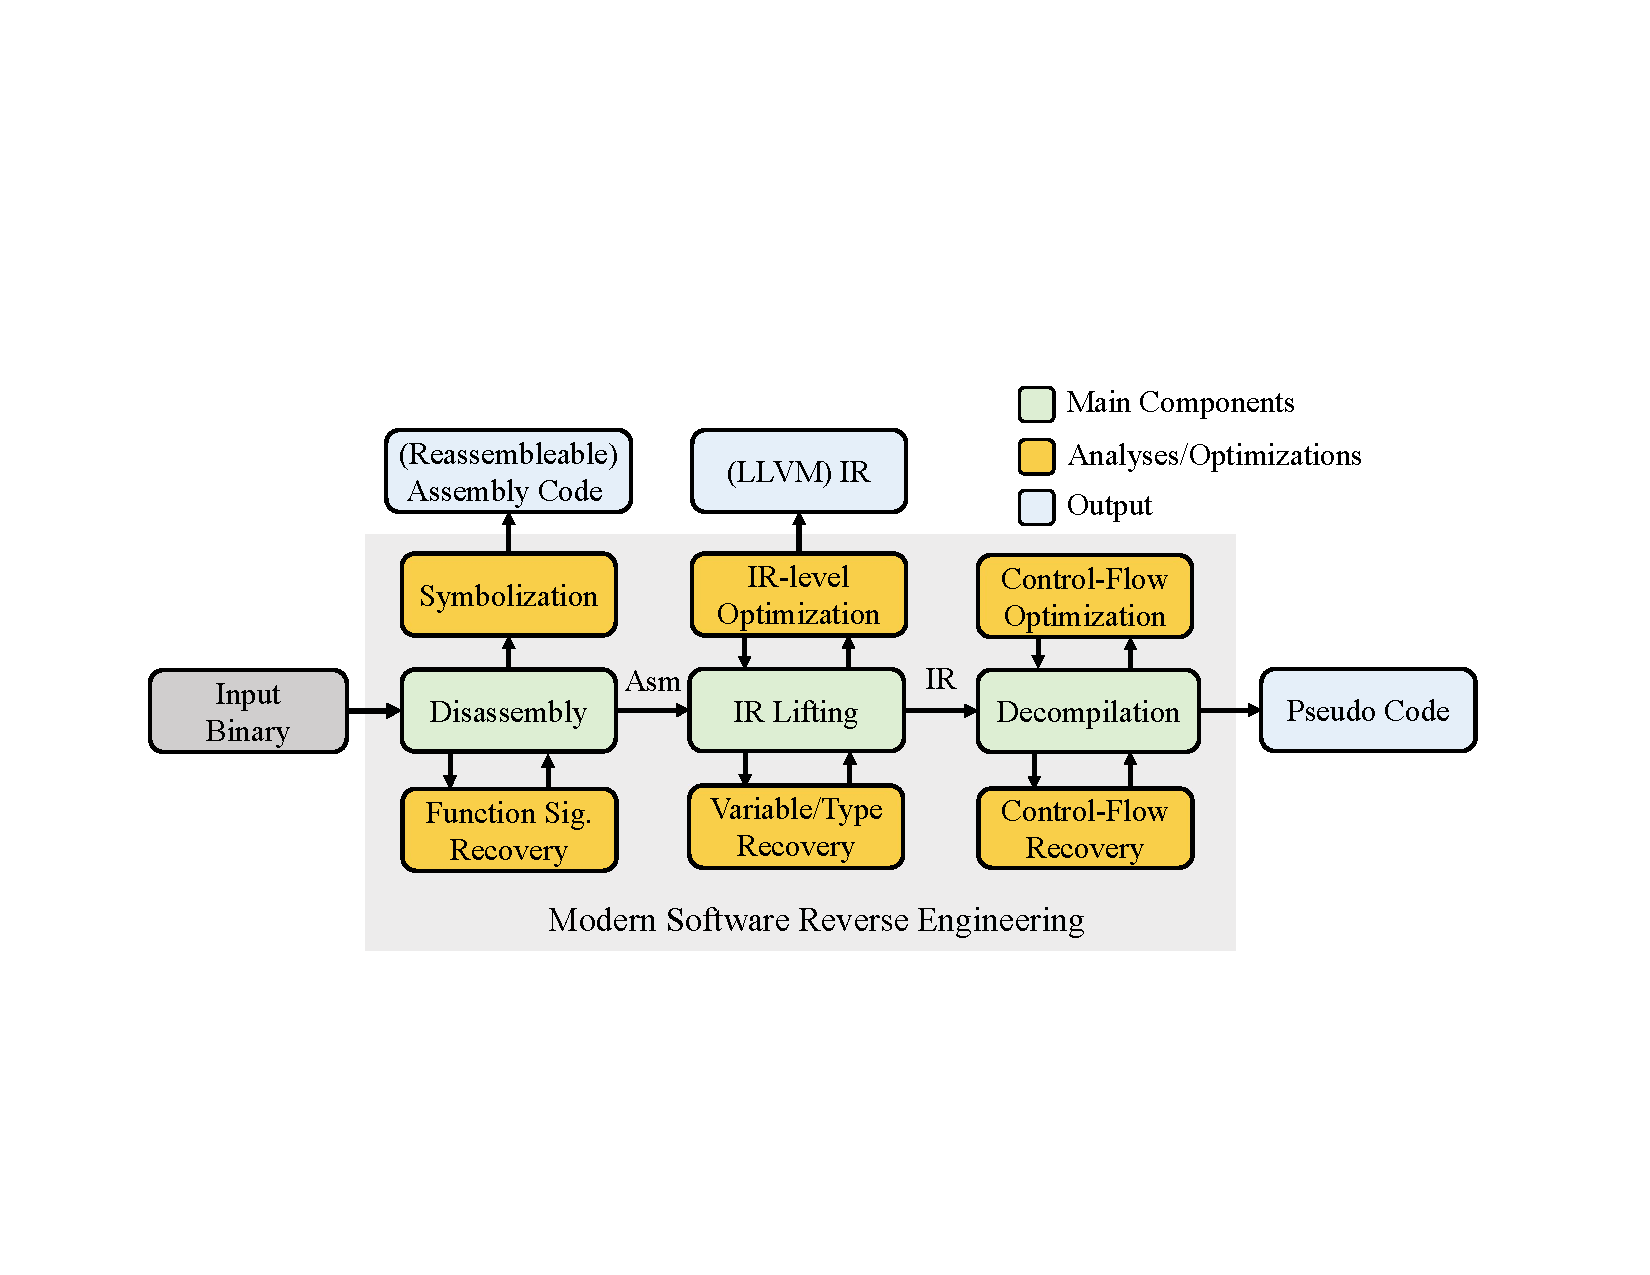
\includegraphics[width=1.0\textwidth]{fig/workflow.pdf}
  \caption{Workflow of modern software reverse engineering.}
  \label{fig:workflow}
\end{figure}

% structure

To be more specific, we first introduce the basic concepts, workflow, and vast
applications of software reverse engineering. Following the workflow, we then
present the challenges of software reverse engineering with the SOTA solutions.
In the end, we discuss the emerging field of decompilation research and some
potential research directions for further improving the capacity of software
reverse engineering.


\newpage
